\section{Introduction}

\section{Popper-compliant Papers}

% what papers have we done
We have authored five Popper-compliant papers:
\begin{itemize}

\item quiho: Automated Performance Regression Testing Using Inferred
Resource Utilization Profiles~\cite{}

\item Cudele: An API and Framework for Programmable Consistency and
Durability in a Global Namespace~\cite{sevilla:ipdps18-cudele}

\item Malacology: A Programmable Storage
System~\cite{sevilla:eurosys17-malacology}

\item Characterizing and Reducing Cross-Platform Performance Using
OS-level Virtualization

\item Programmable Caches with a Data Management Language \& Policy Engine

\end{itemize}

We use the reader/reviewer sample workflow outlined
in~\cite{jimenez:ipdpsw17-popper} and shown in Figure~\ref{fig:workflow}. For
the visualization component (1), we use Jupyter notebooks. The notebooks
themselves are versioned with Git and users interact with local copies by
cloning the repository and launching a Jupyter Docker container. The paper is
written in \LaTeX and built with a Docker container.  For the code component
(2), both the source code for the system itself and the deploy/experiment code
is stored on GitHub. When running experiments, we use Docker containers to
isolate libraries and binaries. For the multi-node component (3), we use
CloudLab machines and Ansible to script deployment and experiment
orchestration. For the data set components (4), we use GitHub to store results
files; our inputs and results are small enough that we do no need a larger
capacity.  GitHub allows files up to 50MB and stores data on S3.

\begin{figure}[tb] 
  \centering
  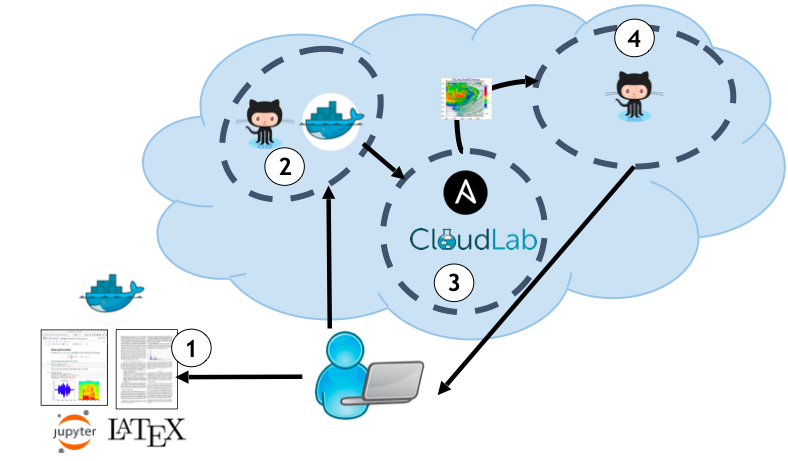
\includegraphics[width=1\linewidth]{./figures/workflow.png}
  \caption{Illustration of the Popper workflow used in our papers; Figure is
adapted from~\cite{jimenez:ipdpsw17-popper}. For (1) - the visualization
component - we use Jupyter, \LaTeX, and Docker; for (2) - the code component -
we use GitHub and Docker; for (3) - the multi-node component - we use Ansible
and CloudLab; and for (4) - the data set component - we use GitHub.}
  \label{fig:workflow}
\end{figure}

Our experiments start with a baseline; to describe the process, we reference
our
\href{https://github.com/michaelsevilla/ceph-popper-template}{ceph-popper-template}
set up on CloudLab. Users setup SSH keys and deploy CloudLab nodes using our
\href{https://www.cloudlab.us/p/CephFS/CephFS-HEP}{CephFS Profile}.  The
profile has the nodes automatically install Docker on bootup using our
\href{https://github.com/michaelsevilla/ceph-popper-template/blob/master/hardware/cloudlab/install.sh}{install}
script. After the nodes finish booting (i.e.  their status on the CloudLab GUI
read as READY), users push SSH keys using a convenience
\href{https://raw.githubusercontent.com/michaelsevilla/ceph-popper-template/master/hardware/cloudlab/pushkeys.sh}{script}.

The deploy code is based on
\href{https://github.com/ceph/ceph-ansible/wiki}{ceph-ansible}, a tool that
configures hardware and software for Ceph. We forked the project and made it
less dependent on Python. To run an experiment, users log in into the head node
and clone the ceph-popper-template. This repository has submodules that point
to ceph-ansible and our own custom roles; configuration files for our Ceph
setup; and helper scripts written in bash that deploy Ceph and run the
benchmarks. For more information, see the
\href{https://github.com/michaelsevilla/ceph-popper-template}{README}. For more
information on the baseline and pipelines terminology, read more on the
\href{http://falsifiable.us/}{Popper Convention}. Then users configure their
cluster by specificing IPs and user names in the \texttt{hosts} file. 

Finally, users specify the Ceph services that should be deployed using the
\href{https://github.com/michaelsevilla/ceph-popper-template/tree/master/pipelines/baseline/ansible}{\texttt{ansible/}}
directory. This directory has code for deploying Ceph and its components:
\texttt{ansible.cfg}, \texttt{ceph.yml}, \texttt{cleanup.yml},
\texttt{group\_vars}, \texttt{monitor.yml}, and \texttt{workloads}. The *.yml
files are Ansible playbooks that start and configure components: ceph.yml
starts Ceph, cleanup.yml tears Ceph down, and monitor.yml starts daemons that
monitor performance. We separate these components into different playbooks so
users can mix and match Ceph services. The workloads directory has scrips for
running the baseline benchmarks. The other files and directories are Ansible
configuration files used by the playbooks.

Users can change the ansible/ceph.yml to specify which Ceph daemons to launch
in the cluster. It uses the hosts file we set up above and is based off the
ceph-ansible site file. High level configurations are in the vars.yml. This
file is heavily commented. For CloudLab, uncomment all blocks labeled
``Uncomment for CloudLab".

To configure the Ceph cluster with the variables in the Ceph configuration file
\href{http://docs.ceph.com/docs/jewel/rados/configuration/ceph-conf/}{documentation},
change the Ansible \texttt{group\_vars/all} file. We also need to specify the
Docker image. These can be specified in each configuration file for the daemon
but for simplicity we put everything in the global variable file. Finally,
users run the \texttt{run.sh} script. 


%% describe paper repository
%As an example, we use our Cudele publication~\cite{sevilla:ipdps18-cudele}. 
%
%
%\noindent \textbf{Paper Directory}: The
%\href{https://github.com/systemslab/cudele-popper/tree/master/paper}{paper
%directory} houses figures, bibliography, and \LaTeX source code. We use a
%common
%\href{https://github.com/michaelsevilla/biblio/tree/ee5f0d6744945fbcc5ddeaf8f5dbb86e1b8f8353}
%{bibliography} across papers, maintained in a separate repository so we have a
%submodule linked. The
%\href{https://github.com/systemslab/cudele-popper/blob/master/paper/build.sh}{build}
%script launches a \LaTeX Docker container and builds the PDF; different PDF
%versions, including our revisions and rebuttals can also be found in this
%`paper` directory.\\
%
%\noindent \textbf{Experiment Directory}: The
%\href{https://github.com/systemslab/cudele-popper/tree/master/experiments}{experiment
%directory} has all the experimental setup scripts, results, and visualizations.
%For example, the
%\href{https://github.com/systemslab/cudele-popper/tree/master/experiments/cudele-mergescale}{merge
%scale} experiment, in addition to the Popper \texttt{*.sh} script, has the
%following directories:
%
%\begin{itemize}
%  \item \texttt{ansible/}: experiment-specific deploy and benchmarking code, written in Ansible
%  \item \texttt{configs\_*/}: configuration code for CloudLab and our internal cluster named Piha.
%  \item \texttt{docker/}: experiment-specific images for housing and distributing source code
%  \item \texttt{results-*/}: results produced by the \texttt{run.sh} script
%  \item \texttt{visualize/}: Jupyter notebooks for viewing and interacting with results`
%\end{itemize}
%
%The actual workflow is shown in Figure~\ref{}. Users change to the directory,
%configure their cluster (using hte \texttt{configs\_*/} directory and
%\texttt{hosts} )

% degrees of popperization

\section{Reproducibility Must Be a 1st Class Citizen}
% exploration vs. complete
% cross-cluster compatibility 
%  - inventory files hard coded throughout tree
%  - configuration files not propagated for experiments
%  - visualize files pulled data from hard coded paths
%  - graphs not created automatically
% why Mantle failed

\section{Organized Repositories and Documentation}
%cause the most work
% role of git
% docker images saved in internal registry (buildding)

\section{Well-Defined Collaboration Roles}
% keeping organization
% workflows

\section{Maintaining Pointers}
% wary of ephemeral links

% large code bases large code bases (src, deploy)

% different registry hubs (Docker, GitHub)

\section{Conference Requirements}
% double blinded??
% private systems?

\section{Conclusion}
